\documentclass{article}
\usepackage{tikz,pgfplots}
%\pgfplotsset{colormap={mix}{
%	color(0cm)=(blue);
%	color(1cm)=(green);
%	color(2cm)=(yellow)
%	color(3cm)=(red)}}

\usetikzlibrary{patterns}

\definecolor{diplom1}{rgb}{0.0 0.4 1.0}
\definecolor{diplom2}{rgb}{0.0 0.0 0.6}
\definecolor{diplom3}{RGB}{153,0,0} %unirot
\definecolor{diplom4}{RGB}{232,215,23}
\definecolor{diplom5}{RGB}{51,37,60}

\definecolor{unirot}{RGB}{153,0,0}
\definecolor{unirot_hell}{RGB}{255,228,225}
\definecolor{lightblue}{RGB}{242.2,249.88,255}

\pgfplotsset{colormap={diplom1s}{
       color(0cm)=(white);
       color(1cm)=(diplom1);
       color(10cm)=(diplom1)}}
\pgfplotsset{colormap={diplom2s}{
       color(0cm)=(white);
       color(1cm)=(diplom1);
       color(2cm)=(diplom2)}}


\newenvironment{customlegend}[1][]{%
    \begingroup
    \csname pgfplots@init@cleared@structures\endcsname
    \pgfplotsset{#1}%
}{%
    \csname pgfplots@createlegend\endcsname
    \endgroup
}%
\def\addlegendimage{\csname pgfplots@addlegendimage\endcsname}

\newcommand{\addlegendimageintext}[1]{%
    \tikz {
        \begin{customlegend}[
            legend entries={\empty},
            legend cell align=left,
            legend style={
                draw=none,
                inner sep=0pt,
                column sep=0pt,
                nodes={inner sep=0pt}}]
        \addlegendimage{#1}
        \end{customlegend}
    }%
}


\begin{document}

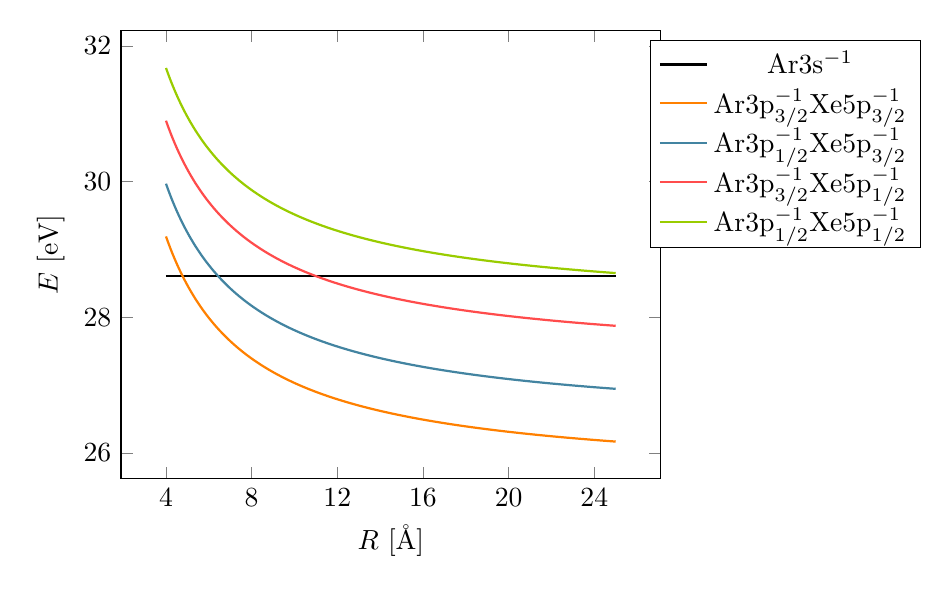
\begin{tikzpicture}
    \begin{axis}[domain=4.0:25,
                 samples = 200,
                 xtick={4.0,8.0,...,24},
                 %xticklabels={$-\pi$,$-\frac \pi 2$,0,$\frac \pi 2$,$\pi$},
                 cycle list name = exotic,
                 legend style={anchor= north west},
                 xlabel={$R$ [\AA]},
                 ylabel={$E$ [eV]}
                 ]
      \addplot+[
                mark = none,
                black,
                thick
               ]
               {29.239 - 0.636};
      \addlegendentry{Ar3s$^{-1}$};
      \addplot+[
                mark = none,
                thick
               ]
               {15.7596 - 1.0 + 12.1298 - 1.3 + 14.39964 / x};
      \addlegendentry{Ar3p$_{3/2}^{-1}$Xe5p$_{3/2}^{-1}$};
      \addplot+[
                mark = none,
                thick
               ]
               {15.9371 - 0.4 + 12.1298 -1.3 + 14.39964 / x};
      \addlegendentry{Ar3p$_{1/2}^{-1}$Xe5p$_{3/2}^{-1}$};
      \addplot+[
                mark = none,
                thick
               ]
               {15.7596 - 1.0 + 13.4363 -0.9 + 14.39964 / x};
      \addlegendentry{Ar3p$_{3/2}^{-1}$Xe5p$_{1/2}^{-1}$};
      \addplot+[
                mark = none,
                thick
               ]
               {15.9371 -0.4 + 13.4363 - 0.9 + 14.39964 / x};
      \addlegendentry{Ar3p$_{1/2}^{-1}$Xe5p$_{1/2}^{-1}$};
      %\draw[] (axis cs:\pgfkeysvalueof{/pgfplots/xmin},29.239) -- (axis cs:\pgfkeysvalueof{/pgfplots/xmax},29.239);
    \end{axis}
\end{tikzpicture}

\end{document}
